\documentclass{beamer}
\usepackage{graphicx}
\usepackage{xcolor}
\usepackage{tikz}
\usepackage{amsmath}

\definecolor{purpleblue}{RGB}{80, 80, 180}
\definecolor{novelPurple}{RGB}{98, 54, 255}
\definecolor{softPurple}{RGB}{180, 170, 255}
\definecolor{softGray}{RGB}{235, 235, 245}
\definecolor{lightText}{RGB}{90, 90, 110}

\usetheme{Madrid}
\usecolortheme{dolphin}
\graphicspath{{static/course_materials/}{static/hard/}{./}}

\setbeamerfont{title}{size=\Large,series=\bfseries}
\setbeamerfont{frametitle}{size=\LARGE,series=\bfseries}
\setbeamercolor{frametitle}{fg=white, bg=novelPurple}
\setbeamercolor{title}{fg=white, bg=purpleblue}

\title[SAT Hard Question 3]{\textbf{SAT Hard Question\\ Set 3}}
\author{\textbf{Jack Zeng}}
\institute{\textcolor{white}{\textbf{Novel Prep}}}
\date{\today}

\begin{document}

\begin{frame}
    \titlepage
    \vfill
    \begin{flushright}
        \textcolor{purpleblue}{\Huge \textbf{Novel Prep}}
    \end{flushright}
\end{frame}

\begin{frame}
    \begin{tikzpicture}[remember picture, overlay]
        \shade[top color=softPurple, bottom color=softGray]
            (current page.north west) rectangle (current page.south east);
        \node[align=center] at (current page.center) {
            {\Huge\bfseries\textcolor{purpleblue}{Novel Prep}} \\[0.5cm]
            {\Large\itshape\textcolor{lightText}{Phase 2 · Hard Question Practice}}
        };
    \end{tikzpicture}
\end{frame}

\begin{frame}{Overview}
    \tableofcontents
\end{frame}

\begin{frame}
\section{Hard Question Set 3}
    \begin{tikzpicture}[remember picture, overlay]
        \shade[top color=softPurple, bottom color=softGray]
            (current page.north west) rectangle (current page.south east);
        \node[align=center] at (current page.center) {
            {\LARGE\bfseries\textcolor{purpleblue}{Hard Question Set 3}} \\[0.5cm]
            {\Large\itshape\textcolor{lightText}{5 SAT-style challenge problems}}
        };
    \end{tikzpicture}
\end{frame}

% --- Question 1 ---
\begin{frame}{Question 1}
\small
A research manager selected 2 random samples of ovens of a certain type to estimate the average amount of time this type of oven takes to preheat to \(325^\circ F\). The research manager recorded the amount of time, in minutes, each oven takes to preheat to \(325^\circ F\).

Based on the first sample, the manager estimated an average of 14.2 minutes, with a margin of error of 1 minute. Based on the second sample, the estimate was 14.4 minutes, with a margin of error of 2.3 minutes.

Assuming the margins of error were calculated the same way, which of the following best explains why the first sample had a smaller margin of error?
\vspace{0.35cm}
\begin{enumerate}
    \item[A.] The first sample contained fewer ovens than the second sample.
    \item[B.] The first sample contained more ovens than the second sample.
    \item[C.] The first sample took less time on average to preheat.
    \item[D.] The first sample took more time on average to preheat.
\end{enumerate}
\end{frame}
\begin{frame}{Answer 1}
\small
\textbf{Correct Answer:} B
\end{frame}

% --- Question 2 ---
\begin{frame}{Question 2}
\small
\begin{center}
    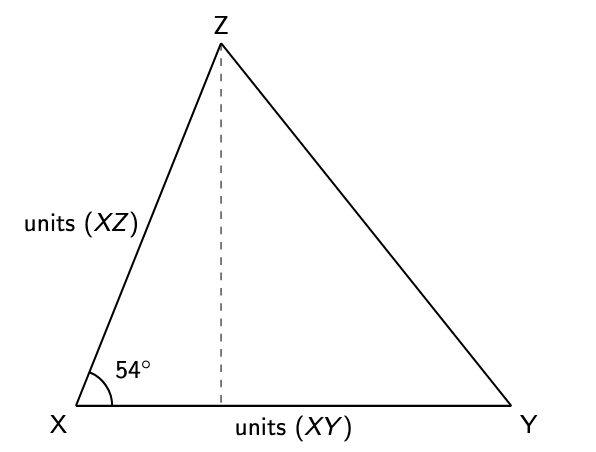
\includegraphics[width=0.45\linewidth]{hard_3_f9.png}
\end{center}

In triangle \(XYZ\), \(\angle X = 54^\circ\), \(XY = 26\) units, \(XZ = 19\) units. What is the area, in square units, of triangle \(XYZ\)?
\vspace{0.35cm}
\begin{enumerate}
    \item[A.] 247
    \item[B.] 494
    \item[C.] \(247\sin 54^\circ\)
    \item[D.] \(494\sin 54^\circ\)
\end{enumerate}
\end{frame}
\begin{frame}{Answer 2}
\small
\textbf{Correct Answer:} C
\end{frame}

% --- Question 3 ---
\begin{frame}{Question 3}
\small
In the figure, \(\triangle ABC\) is inscribed in a semicircle with diameter \(AC = 10\). Point \(B\) lies on the semicircle. If \(AB = 6\) and \(BC = x\), find \(x\). Give your answer in simplest radical form.
\vspace{0.35cm}
\begin{enumerate}
    \item[A.] \(\sqrt{36}\)
    \item[B.] 8
    \item[C.] \(\sqrt{44}\)
    \item[D.] \(\sqrt{64}\)
\end{enumerate}
\end{frame}
\begin{frame}{Answer 3}
\small
\textbf{Correct Answer:} B
\end{frame}

% --- Question 4 ---
\begin{frame}{Question 4}
\small
A parabola is given by
\[
y = x^2 - 4x + 5,
\]
and a circle by
\[
x^2 + y^2 = 25.
\]

The parabola and circle intersect at points \(P\) and \(Q\). Find the distance between \(P\) and \(Q\).
\end{frame}
\begin{frame}{Answer 4}
\small
\textbf{Final Answer:} $\boxed{3.88}$
\end{frame}

% --- Question 5 ---
\begin{frame}{Question 5}
\small
Solve the equation:
\[
\sqrt{6r} = \sqrt{r^2 - 16}
\]

What is the product of all solutions to the above equation?
\vspace{0.35cm}
\begin{enumerate}
    \item[A.] 4
    \item[B.] 6
    \item[C.] 8
    \item[D.] 12
\end{enumerate}
\end{frame}
\begin{frame}{Answer 5}
\small
\textbf{Correct Answer:} C
\end{frame}

\begin{frame}{}
    \begin{tikzpicture}[remember picture, overlay]
        \shade[top color=novelPurple!40, bottom color=white]
            (current page.north west) rectangle (current page.south east);
        \fill[white, opacity=0.15] (current page.center) circle (5cm);
        \foreach \x in {1,2,3,4,5} {
            \fill[novelPurple, opacity=0.12] (rand*10-5, rand*7-3.5) circle (0.1+\x*0.05);
        }
    \end{tikzpicture}
    \centering
    \vspace{5em}
    {\Huge \textbf{\textcolor{novelPurple}{Thank You!}}} \\[1em]
    {\large \textcolor{gray}{We appreciate your time and focus.}} \\[3em]
    {\LARGE \textbf{\textcolor{novelPurple}{\textsf{Novel Prep}}}}
    \vfill
\end{frame}

\end{document}
